\documentclass[A4]{article}
\usepackage[T2A]{fontenc}
\usepackage{fontspec}
\setmainfont{CMU Serif}
\usepackage{amsmath}
\usepackage{amssymb}
\usepackage[russian]{babel}
\usepackage{xeCJK}% 调用 xeCJK 宏包
\usepackage{booktabs}
\usepackage{multirow}
\usepackage{graphicx}
\usepackage{listings}
\usepackage{bm}
\usepackage{geometry}
\geometry{a4paper,scale=0.8}
\usepackage[pdfborder=000]{hyperref}
\usepackage[usenames,dvipsnames]{xcolor}
\setCJKmainfont{SimHei}

\begin{document}
\author{Сюй Минчуань}
\title{Математические Основы Теории Управления}
\maketitle
 \tableofcontents
\newpage
\section{Теория управления}
\textbf{Объект управления} (управляемый объект) - это динамический объект, на который можно оказывать целенаправленное (управляющее) воздействие.\\
\bm{$u(t)$} - вектор управляющих (входных) воздействий.\\
\bm{$f(t)$} - вектор возмущающих воздействий (паразитные возмущения или полезная нагрузка).\\
\bm{$x(t)$} - вектор переменных состояния.\\
\bm{$y(t)$} - вектор регулируемых (выходных) переменных.\\
\\
\textbf{Структура системы управления}\\
объект управления (ОУ)\\
задающее устройство (ЗУ)\\
регулирующее (управляющее) устройство (УУ)\\
эталонная модель (ЭМ) - $y_m=F(G)$\\
$e$ - ошибка управления \\

\begin{figure}[htbp] 
	\centering 
	\begin{minipage}[t]{0.48\textwidth} 
		\centering 
		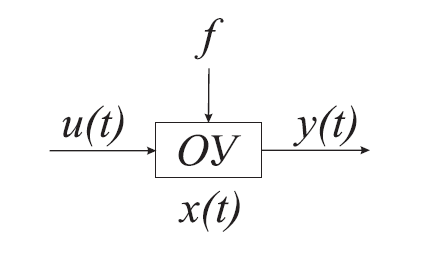
\includegraphics[width=5cm]{1} 
		\caption{Объект управления}
		\label{fig:1}
	\end{minipage} 
	\begin{minipage}[t]{0.48\textwidth} 
		\centering 
		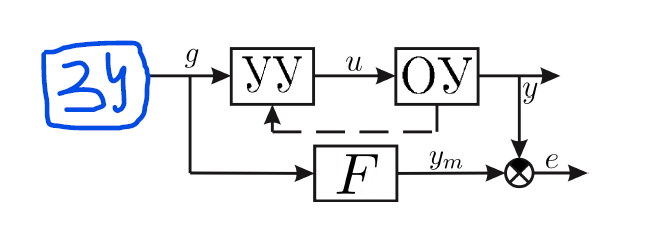
\includegraphics[width=5cm]{2} 
		\caption{Структура системы управления} 
		\label{fig:2}
	\end{minipage} 
\end{figure}

\noindent Различают два типа управления:\\
\emph{Управление по разомкнутому контуру} - текущее состояния объекта не влияет.\\
\emph{Управление по замкнутому контуру} - управление с обратной связью.
\begin{figure}[htbp] 
	\centering 
	\begin{minipage}[t]{0.48\textwidth} 
		\centering 
		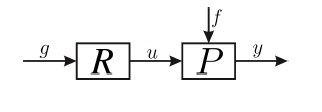
\includegraphics[width=5cm]{3} 
		\caption{Управление по разомкнутому контуру}
		\label{fig:3}
	\end{minipage} 
	\begin{minipage}[t]{0.48\textwidth} 
		\centering 
		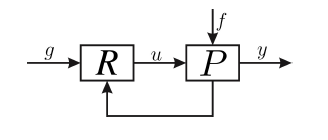
\includegraphics[width=5cm]{4} 
		\caption{Управление по замкнутому контуру} 
		\label{fig:4}
	\end{minipage} 
\end{figure}
\\
\textbf{Примеры математического представления динамических систем}
\begin{itemize}
	\item С помощью \textbf{дифференциальных уравнений}
	\begin{equation}
	\left\{\begin{array}{cc}
	\dot{x}=f(x,u),\\
	\dot{y}=h(x,u).\\
	\end{array}\right.
	\end{equation}
	\begin{equation}
	\left\{\begin{array}{cc}
	F(x_1,\ldots,x_n,\ldots,x_1^{(m)},\ldots,x_n^{(m)},\ldots,u,\ldots,u^{(k)})=0,\\
	y=h(x,u).\\
	\end{array}\right.
	\end{equation}
	\begin{equation}
	F(y,\dot{y},\ldots,y^{(m)},u^{(0)},\ldots,u^{(k)})=0
	\end{equation}
	\item С помощью \emph{интегральных уравнений} $y(t)=\int_{0}^{t} K(t,\tau)u(\tau)d\tau$
	\item С помощью \textbf{передаточной функции} $Y(s)=W(s)U(s)$
	\item С помощью \textbf{структурных схем} $x([k+1]T)=f(x[kT],u[kT])$
	\item С помощью \textbf{разностных уравнений}
\end{itemize}

\textbf{Классификация динамических систем}
\begin{itemize}
	\item Непрерывные и дискретные
	\item Линейные и нелинейные
	\item Конечномерные и бесконечномерные
	\item Стационарные и нестационарные - явно входит ли время или нет. 
	\item Скалярные и векторные - входные (выходные) сигналы скалярны или нет. 
\end{itemize}

\textbf{Синтез алгоритмов управления}
\begin{itemize}
	\item \emph{Задача управления состоянием}: найти $u: \forall x_1(0)\stackrel{u}{} x_2(T).x_1\in X_1,x_2\in X_2$.\\
	Частные случаи: \\
	Задача стаблизации состояния: Переводить систему из любого состояния в точку нули за какое-то время.\\
	Задача программного управления: найти $u: \forall x_1\stackrel{u}{} x_2.X_1=\{x_1\},X_2=\{x_2\}$.\\
	\item \emph{Задача управления выходом}: Для заданной эталонной модели $y_m$ построить управление $u:y-y_m \rightarrow 0, t\rightarrow 0$.\\
	Частные случаи: \\
	Задача стаблизации выхода:$g\equiv const$.\\
	Задача программного управления: $g(t)$ заранее известна.\\
	Задача слежения: $g(t)$ заранее неизвестна.\\
	\begin{figure}
		\centering
		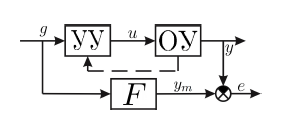
\includegraphics[width=0.7\linewidth]{5}
		\caption{Задача управления выходом}
		\label{fig:5}
	\end{figure}
\end{itemize}

\textbf{Принципы управления}
\begin{itemize}
	\item Принцип программного управления - Об объекте управления все известно, то известна выходная функция. 
	\item Принцип компенсации (управления по возмущению) - В зависимости от возмущения происходит его компенсация. Необходимо измерять возмущения
	\item Принцип обратной связи - Обеспечить стремление ошибки к нулю.
	\item Принцип комбинированного управления - Совместное использование принципа компенации и принципа обратной связи.
\end{itemize}

\section{Линейная теория управления}
\subsection{Линеаризация}
Пусть имеется система уравнений
\begin{equation}
\left\{\begin{array}{cc}
F_1(x,\dot{x},\ddot{x},y,\dot{y},\ddot{y},z,\dot{z},\ddot{z})=0,\\
F_2(x,\dot{x},\ddot{x},y,\dot{y},\ddot{y},z,\dot{z},\ddot{z})=0.\\
\end{array}\right.
\end{equation}
Нас интересует поведение системы при $v_0=(x_0,0,0,y_0,0,0,z_0,0,0)$. Обозначим отклонения через $\Delta x,\Delta y,\Delta z$, тогда $x=x_0+\Delta x,\dot{x}=\Delta\dot{x}, \ddot{x}=\Delta\ddot{x}$. Подставим эти выражения в систему и разложим в ряд Тейлора в окрестности точки
\begin{equation}
\left\{\begin{array}{cc}
F_1(v_0)+\frac{\partial F_1}{\partial x}(v_0)\Delta x+\frac{\partial F_1}{\partial \dot{x}}(v_0)\Delta \dot{x}+\frac{\partial F_1}{\partial \ddot{x}}(v_0)\Delta \ddot{x}+\ldots=0,\\
F_2(v_0)+\frac{\partial F_2}{\partial x}(v_0)\Delta x+\frac{\partial F_2}{\partial \dot{x}}(v_0)\Delta \dot{x}+\frac{\partial F_2}{\partial \ddot{x}}(v_0)\Delta \ddot{x}+\ldots=0.\\
\end{array}\right.
\end{equation}
Учитывая, что $F_1(v_0)=0,F_2(v_0)=0$, и подбрасывая нелинейные слагаемые высшего порядка относительно отклонений, получаем линейные уравнения относительно $\Delta x,\Delta y,\Delta z,\Delta \dot{x},\Delta \dot{y},\Delta \dot{z},\Delta \ddot{x},\Delta \ddot{y},\Delta \ddot{z}$.
\begin{equation}
\left\{\begin{array}{cc}
\frac{\partial F_1}{\partial x}(v_0)\Delta x+\frac{\partial F_1}{\partial \dot{x}}(v_0)\Delta \dot{x}+\frac{\partial F_1}{\partial \ddot{x}}(v_0)\Delta \ddot{x}=0,\\
\frac{\partial F_2}{\partial x}(v_0)\Delta x+\frac{\partial F_2}{\partial \dot{x}}(v_0)\Delta \dot{x}+\frac{\partial F_2}{\partial \ddot{x}}(v_0)\Delta \ddot{x}=0.\\
\end{array}\right.
\end{equation}
\subsection{Методы описания линейных скалярных стационарных непрерывных конечномерных систем(ЛССНКС)}
\subsubsection{Метод пространства состояний}
\begin{equation}
\left\{\begin{array}{cc}
\dot{x}=Ax+bu,x\in \mathbb{R}^n,u,y\in\mathbb{R}^1,t\ge 0,\\
y=cx+du\quad A\in \mathbb{R}^{n\times n},d\in\mathbb{R}^1,b,c^T\in\mathbb{R}^n.\\
\end{array}\right.
\end{equation}
\begin{equation}
\begin{aligned}
x(t)&=e^{At}x(0)+\int_{0}^{t}e^{A(t-\tau)}bu(\tau)d\tau,\\
y(t)&=ce^{At}x(0)+c\int_{0}^{t}e^{A(t-\tau)}bu(\tau)d\tau+du.\\
e^{At}&=I+At+\frac{1}{2!}A^2t^2+\ldots+\frac{1}{n!}A^nt^n+\ldots,\\
\frac{d}{dt}e^{At}&=Ae^{At}.\\
\end{aligned}
\end{equation}
\subsubsection{Невырожденное преобразование пространства состояний}
Пусть имеем невырожденное преобразование $z=Mx,|M|\ne 0$\\
\begin{equation}
\left\{\begin{array}{cc}
\dot{x}=Ax+bu,\\
y=cx+du.\\
\end{array}\right.
\end{equation}
\begin{equation}
\left\{\begin{array}{cc}
\dot{z}=M\dot{x}=M(Ax+bu),z(0)=Mx(0)\\
y=cM^{-1}z+du.\\
\end{array}\right.
\end{equation}
\begin{equation}
\left\{\begin{array}{cc}
\dot{z}=\tilde{A}x+\tilde{b}u,\\
y=\tilde{c}x+du.\\
\end{array}\right.
\end{equation}
где $\tilde{A}=MAM^{-1},\tilde{b}=Mb,\tilde{c}=cM^{-1}$
\subsubsection{Преобразование Лапласа}
Функция оригиналы $f(t)$:\\
1. $f(t)$ - интегрируема на любом конечном $[0,T^*]$;\\
2. $\exists M,\sigma>0:|f(t)|\le Me^{\sigma t},t\ge 0$.\\
Тогда применимо \emph{преобразование Лапласа}:\\ $\mathcal{L}\{f(t)\}=\int_{0}^{\infty} f(t)e^{-st}dt=F(s),s=\alpha+i\beta$ - комплесный параметр.\\
\\
Свойства преобразования Лапласа
\begin{itemize}
	\item $\alpha_1f_1(t)+\alpha_2f_2(t)\risingdotseq\alpha_1F_1(s)+\alpha_2F_2(s)$
	\item $f^{(k)}\risingdotseq s^kF(s)-s^{k-1}f(0)-s^{k-2}f'(0)-\ldots-f^{(k-1)}(0)$
	\item $\int_{0}^{t} f(\tau) d\tau \risingdotseq\frac{F(s)}{s}$//
	Подробно (также таблицу ) см. лекцию
\end{itemize}
\subsubsection{Нахождение оригиналов по изображениям Лапласа}
Пусть $Y(s)=\frac{\gamma(s)}{\mu(s)}$
\begin{itemize}
	\item $\mu(s)$ имеет простые корни $s_1,\ldots,s_n$, тогда
	\begin{equation}
	y(t)=\sum_{i=1}^{n}\frac{\gamma(s_i)}{\mu'(s_i)}e^{s_i t}	
	\end{equation} 
	\item $\mu(s)$ имеет кратные корни
	\subitem $\frac{A}{(s-s_0)^k}\fallingdotseq Ae^{s_0t}\frac{t^{k-1}}{k!}$
	\subitem $\frac{As+B}{(s^2+Cs+D)^k}$ к примеру:
	\begin{equation}
	\frac{s+2}{s^2-2s+2}=\frac{s+2}{(s-1)^2+1}=\frac{s-1}{(s-1)^2+1}+\frac{3}{(s-1)^2+1}\fallingdotseq e^t\cos t+3e^t\sin t
	\end{equation}
\end{itemize}
\subsubsection{Метод передаточной функции (Переход от ПС к ПФ)}
\begin{equation}
\left\{\begin{array}{cc}
\dot{x}=Ax+bu,\\
y=cx.\\
\end{array}\right.
\end{equation}
Будем считать, что $x(0)=0$. Применим к уравнению состояния и уравнению выхода преобразования Лапласа, преобразуем и получим \emph{передаточную функцию}.
\begin{equation}
\left\{\begin{array}{cc}
sX(s)-x_0=AX(s)+bU(s),\\
Y=cX\\
\end{array}\right.
\end{equation}
Описание через передаточную функцию:\\ $Y(s)=W(s)U(s),W(s)=c(sI-A)^{-1}b$.\\
Определение. 
\begin{equation}
W(s)=\frac{Y(s)}{U(s)}\bigg|_{x(0)=0}=c(sI-A)^{-1}b=\frac{c(sI-A)^*b}{\det(sI-A)}=\frac{\beta(s)}{\alpha(s)}.
\end{equation}
$\deg \alpha(s)=n$ - динамический порядок объекта.\\
$\deg \beta(s)=m$.\\
$r=n-m$ - относительный порядок объекта.\\
$r\ge 0$ - физически реализуемая,\\
$r>0$ - строго физически реализуемая,\\
$r<0$ - физически нереализуемая,\\
В случае $d\ne 0$:
\begin{equation}
W(s)=c(sI-A)^{-1}b+d
\end{equation}
\subsubsection{Инвариантность передаточных функций относительно преобразований фазового пространства.}
Пусть имеем невырожденное преобразование $z=Mx,|M|\ne 0$\\
\begin{equation}
\left\{\begin{array}{cc}
\dot{x}=Ax+bu,\\
y=cx.\\
\end{array}\right.
\end{equation}
\begin{equation}
\left\{\begin{array}{cc}
\dot{z}=\tilde{A}x+\tilde{b}u,\\
y=\tilde{c}x+du.\\
\end{array}\right.
\end{equation}
где $\tilde{A}=MAM^{-1},\tilde{b}=Mb,\tilde{c}=cM^{-1}$.\\
$(c,A,b) \leftrightarrow (c,\tilde{A},\tilde{b}) \Rightarrow W(s)=\tilde{W}(s)$.
\subsubsection{Сокращение передаточных функций}
В передаточной функции сокращать можно только \emph{устойчивые множители}. Путем сокращения приходим к новой передаточной фукнции некоторой подсистемы исходной системы.
\subsubsection{Метод ОДУ n-го порядка}
\begin{equation}
y^{(n)}+a_{n-1}y^{(n-1)}+\ldots+a_1\dot{y}+a_0y=b_mu^{(m)}+\ldots+b_1\dot{u}+b_0 u
\end{equation}
\subsubsection{Переход от ПФ к ОДУ}
Пример
\begin{equation}
\begin{aligned}
W(s)=\frac{b_2s^2+b_1s+b_0}{s^2+a_1s+a_0}=\frac{Y(s)}{U(s)},\quad (s^2+a_1s+a_0)Y(s)=(b_2s^2+b_1s+b_0)U(s)\\
(s^2Y(s)-sy(0)-\dot{y}(0))+a_1(sY(s)-y(0))+a_0Y(s)+\bm{sy(0)+\dot{y}(0)+a_1y(0)}=\\b_2(s^2U(s)-su(0)-\dot{u}(0))+b_1(sU(s)-u(0))+b_0U(s)+\bm{b_2su(0)+b_2\dot{u}(0)+b_1u(0)}\\
\end{aligned}
\end{equation}
Пусть выполнено равенство (условие), ищем оригиналы уравнения
\begin{equation}
\left\{\begin{array}{cc}
\ddot{y}+a_1\dot{y}+a_0y=b_2\ddot{u}+b_1\dot{u}+b_0u,\\
y(0)=b_2u(0),\\
\dot{y}(0)=(b_1-a_1b_2)u(0)+b_2\dot{u}(0)\\
\end{array}\right.
\end{equation}
\subsubsection{Переход от ОДУ к ПФ}
Пример
\begin{equation}
\begin{aligned}
\ddot{y}+a_1\dot{y}+a_0y&=b_1\dot{u}+b_0u\quad\quad\risingdotseq\\
s^2Y(s)+a_1sY(s)+a_0Y(s)&=b_1sU(s)+b_0U(s)+\underbrace{\bm{sy(0)+\dot{y}(0)+a_1y(0)-b_1u(0)}}_{=0}
\end{aligned}
\end{equation}
После этого получим
\begin{equation}
\left\{\begin{array}{cc}
Y(s)=\frac{b_1s+b_0}{s^2+a_1s+a_0}U(s),\\
y(0)=0,\\
\dot{y}(0)=b_1u(0).\\
\end{array}\right.
\end{equation}
\subsubsection{Переход от ОДУ к ПC}
Пусть имеем ОДУ
\begin{equation}
\ddot{y}+a_1\dot{y}+a_0y=b_2\ddot{u}+b_1\dot{u}+b_0u
\end{equation}
Предположим
\begin{equation}
\left\{\begin{array}{cc}
y=x_1+k_1u,\\
\dot{x_1}=x_2+k_2u,\\
\dot{x_2}=-a_0x_1-a_1x_2+k_3u
\end{array}\right.
\end{equation}
Найдем $k_i$:
\begin{equation}
\left\{\begin{array}{cc}
y=x_1+k_1u,\quad\Rightarrow x_1=y-k_1u\\
\dot{y}=x_2+k_2u+k_1\dot{u},\\
\ddot{y}=-a_0y-a_1\dot{y}+k_1\ddot{u}+(a_1k_1+k_2)\dot{u}+(a_0k_1+a_1k_2+k_3)u\\
\end{array}\right.
\end{equation}
\begin{equation}
\left\{\begin{array}{cc}
k_1=b_2\\
k_2+a_1k_1=b_1\\
k_3+a_1k_2+a_0k_1=b_0\\
\end{array}\right.
\end{equation}
Из системы уравнений находим $k_i$. Далее, запишем пространство состояний:
\begin{equation}
\left\{\begin{array}{cc}
\dot{x}=Ax+bu,x\in \mathbb{R}^n,u,y\in\mathbb{R}^1,t\ge 0,\\
y=cx+du\quad A\in \mathbb{R}^{n\times n},d\in\mathbb{R}^1,b,c^T\in\mathbb{R}^n.
\end{array}\right.
\end{equation}
где
\begin{equation*}
A=\left(\begin{array}{cc}
0 &1\\
-a_0& -a_1\\
\end{array}\right),b=\left(\begin{array}{c}k_2\\k_3\end{array}\right),\\c=\left(1\quad 0\right),d=k_1
\end{equation*}
$A$ - \emph{матрица Фробениуса}.\\
Согласованность начальных условий:
\begin{equation}
\left\{\begin{array}{cc}
x_1(0)=y(0)-k_1u(0)\\
\dot{y}(0)=x_2(0)+k_2u(0)+k_1\dot{u}(0)
\end{array}\right.
\end{equation}
\subsubsection{Переход от ПФ к ПC}
Пусть $\frac{Y(s)}{\beta(s)}=\frac{U(s)}{\alpha(s)}=X_1(s)$. Рассмотрим $X_1(s)=\frac{U(s)}{\alpha(s)}$.
\begin{equation}
(s^n+a_{n-1}s^{n-1}+\ldots+a_0)X_1=U
\end{equation}
Пусть (Будем считать, что $X_i(0)=0$)
\begin{equation}
\left\{\begin{array}{cc}
sX_1(s)=X_2(s)\\
sX_1(s)=X_3(s)\\
\ldots\\
sX_{n-1}(s)=X_n(s)\\
sX_n(s)=a_0X_1-a_1X_2(s)-\ldots-a_{n-1}X_n(s)+U(s)
\end{array}\right. (\fallingdotseq)\Rightarrow\\
\left\{\begin{array}{cc}
\dot{x_1}=x_2\\
\dot{x_2}=x_3\\
\ldots\\
\dot{x_{n-1}}=x_n\\
\dot{x_n}=-a_0x_1-\ldots-a_{n-1}x_n+u\\
x_i(0)=0,\quad i=1,\ldots,n
\end{array}\right.
\end{equation}
Аналогично (Рассматривая $X_1(s)=\frac{Y(s)}{\beta(s)}$), получим
\begin{equation}
y=b_0x_1+\ldots+b_mx_{m+1}
\end{equation}
Далее, запишем пространство состояний:
\begin{equation}
\left\{\begin{array}{cc}
\dot{x}=Ax+bu,x\in \mathbb{R}^n,u,y\in\mathbb{R}^1,t\ge 0,\\
y=cx\quad A\in \mathbb{R}^{n\times n},b,c^T\in\mathbb{R}^n.\\
\end{array}\right.
\end{equation}
где
\begin{equation*}
A=\left(\begin{array}{ccccc}
0 &1&0&\ldots&0\\
0&0&1&\ldots&0\\
\ldots&\ldots&\ldots&\ldots&\ldots\\
0&0&0&\ldots&1\\
-a_0&-a_1&\-a_2&\ldots&-a_{n-1}\\
\end{array}\right),b=\left(\begin{array}{c}0\\\ldots\\\ldots\\0\\1\end{array}\right),\\c=\left(b_0,\ldots,b_m,0,\ldots,0\right)
\end{equation*}
\subsubsection{Метод интегральных уравнений}
\begin{equation}
\begin{aligned}
Y(s)&=W(s)U(s)\\
&\fallingdotseq\\
y(t)&=\int_{0}^{t}k(t-\tau)u(\tau)d\tau=\int_{0}^{t}k(\tau)u(t-\tau)d\tau
\end{aligned}
\end{equation}
\subsubsection{Метод структурных схем (Переход от СС к ПФ)}
Структурная схема - графическое представление динамического объекта через его подсистемы с указанием связей между ними.\\
\\
\textbf{Основные элемены структурной схемы}
\begin{itemize}
	\item Линия связи - направление распространения сигнала
	\item Точка ветвления - сигнал расходится по линиям связи
	\item Динамическое(статическое) звено
	\item Сумматор
\end{itemize}
\textbf{Основные типы соединений в структурных схемах}
\begin{itemize}
	\item Последовательное соединение
	\item Параллельное соединение
	\item Соединение обратной связью
\end{itemize}
\textbf{Типы преобразований структурных схем}
\begin{itemize}
	\item Декомпозиция - увеличение количества звеньев
	\item Агрегирование - уменьшение количества звеньев
	\item Трансформация - выявление в явном виде основных типов соединений
\end{itemize}
\textbf{Основные правила преобразования структурных схем}
\begin{itemize}
	\item Для агрегировании
	\subitem для последовательного соединения: $y=(w_2w_1)u$
	\subitem для параллельного соединения: $y=(w_1+w_2)u$
	\subitem для соединения обратной связью: $y=\frac{w_1}{1\pm w_1w_2}u$
	\item Для трансформации
	\subitem Перенос точки ветвления через динамическое звено
	\subitem Перенос сумматора
\end{itemize}
\textbf{Алгебраический способ упрощения структурных схем}\\
Проведем проресс упрощения на примере
\begin{equation}
\left\{\begin{array}{cc}
y=\frac{1}{s}(v_1+v_4)\\
v_4=2u\\
v_3=2y\\
v_2=3v_1\\
v_1=\frac{1}{s}(u-v_2-v_3)
\end{array}\right.
\end{equation}
Выразим $y$ через $u$, сокращая $v_1,v_2,v_3,v_4$, получим
\begin{equation}
y=\frac{2s+7}{s^2+3s+2}u
\end{equation}
\subsubsection{Переход от ОДУ к СС}
Описать ОДУ структурной схемой, которая содержит только простейшие элементы.
\begin{equation}
\dddot{y}+a_2\ddot{y}+a_1\ddot{y}+a_0y=b_3\dddot{u}+b_2\ddot{u}+b_1\dot{u}+b_0u
\end{equation}
Его передаточная функция имеет вид:
\begin{equation}
\begin{aligned}
Y(s)&=\frac{b_3s^3+b_2s^2+b_1s+b_0}{s^3+a_2s^2+a_1s+a_0}U(s)\\
\text{Пусть }\bm{Y(s)}&=\bm{(b_2s^2+b_1s+b_0)Y_1(s)}\Rightarrow\\
Y_1(s)&=\frac{1}{s^3+a_2s^2+a_1s+a_0}U(s)\Rightarrow\\
\bm{s^3Y_1(s)}&=\bm{U(s)-a_2s^2Y_1(s)-a_1sY_1(s)-a_0Y_1(s)}\\
\end{aligned}
\end{equation}
\begin{figure}
	\centering
	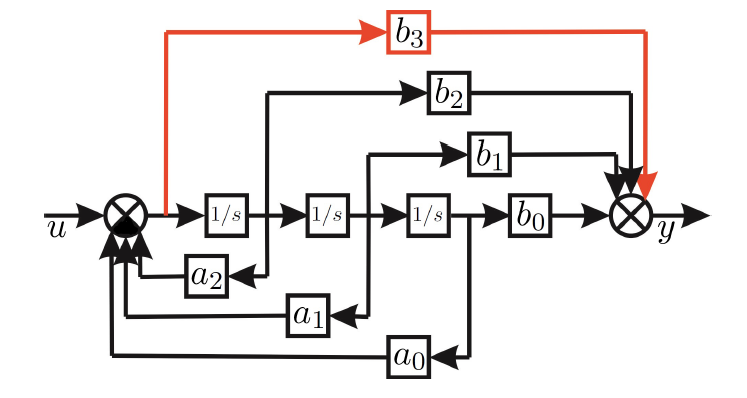
\includegraphics[width=0.7\linewidth]{8}
	\caption{Переход от ОДУ к СС}
	\label{fig:8}
\end{figure}
Другое построение СС из ОДУ (пример):\\
\begin{equation}
\begin{aligned}
\dddot{y}+2\ddot{y}+4\ddot{y}+3y&=7\ddot{u}+5\dot{u}+4u\quad (\risingdotseq)\\
s^3Y+2s^2Y+4sY+3Y&=7s^2U+5sU+4U\\
\end{aligned}
\end{equation}
\begin{equation*}
\bm{Y=\frac{1}{s}\left(-2Y+7U+\frac{1}{s}\left(-4Y+5U+\frac{1}{s}\left(-3Y+4U\right)\right)\right)}
\end{equation*}

\begin{figure}
	\centering
	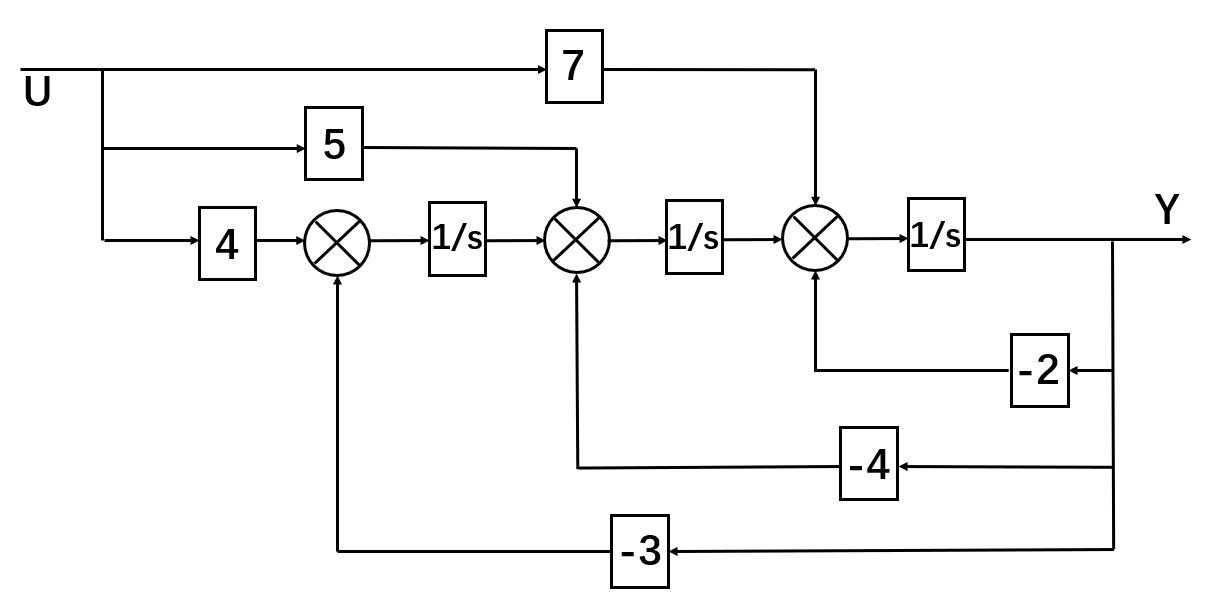
\includegraphics[width=0.7\linewidth]{9}
	\caption{Другое построение СС из ОДУ}
	\label{fig:9}
\end{figure}
\subsubsection{Переход от ПС к СС}
Описать ПС структурной схемой, которая содержит только простейшие элементы. 
\begin{equation}
\left\{\begin{array}{cc}
\dot{x_1}=a_{11}x_1+a_{12}x_2+b_1u\\
\dot{x_2}=a_{21}x_1+a_{22}x_2+b_2u\\
y=c_1x_1+c_2x_2+\mu u
\end{array}\right.\Rightarrow
\left\{\begin{array}{cc}
x_1=1/s(a_{11}x_1+a_{12}x_2+b_1u )\\
x_2=1/s(a_{21}x_1+a_{22}x_2+b_2u)\\
y=c_1x_1+c_2x_2+\mu u
\end{array}\right.
\end{equation}
\begin{figure}
	\centering
	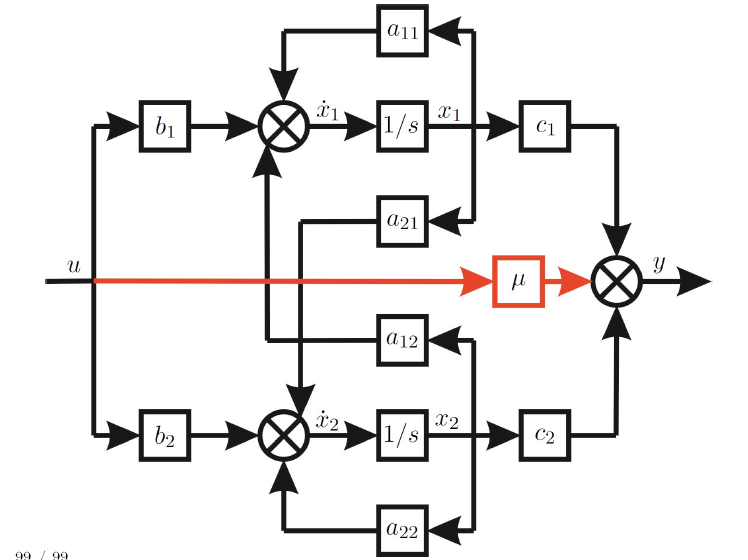
\includegraphics[width=0.7\linewidth]{7}
	\caption{Переход от ПС к СС}
	\label{fig:7}
\end{figure}
\subsubsection{Переход от ПФ к СС}
Описать ПФ структурной схемой, которая содержит только простейшие элементы. (пример )
\begin{equation}
\begin{aligned}
W(p)&=\frac{5p+4}{p^3+2p^2+4p+3}=\frac{5p+4}{(p+1)(p^2+p+3)}=\frac{-1/3}{p+1}+\frac{1/3p+5}{p^2+p+3}\\
Y_1&=\frac{-1/3}{p+1}U\quad\Rightarrow \bm{Y_1=\frac{1}{p}\left(-Y_1-\frac{1}{3}U\right)}\\
Y_2&=\frac{1/3p+5}{p^2+p+3}U\quad\Rightarrow \bm{Y_2=\frac{1}{p}\left(-Y_2+\frac{1}{3}U+\frac{1}{p}\left(-3Y_2+5U\right)\right)}
\end{aligned}
\end{equation}
\begin{figure}
	\centering
	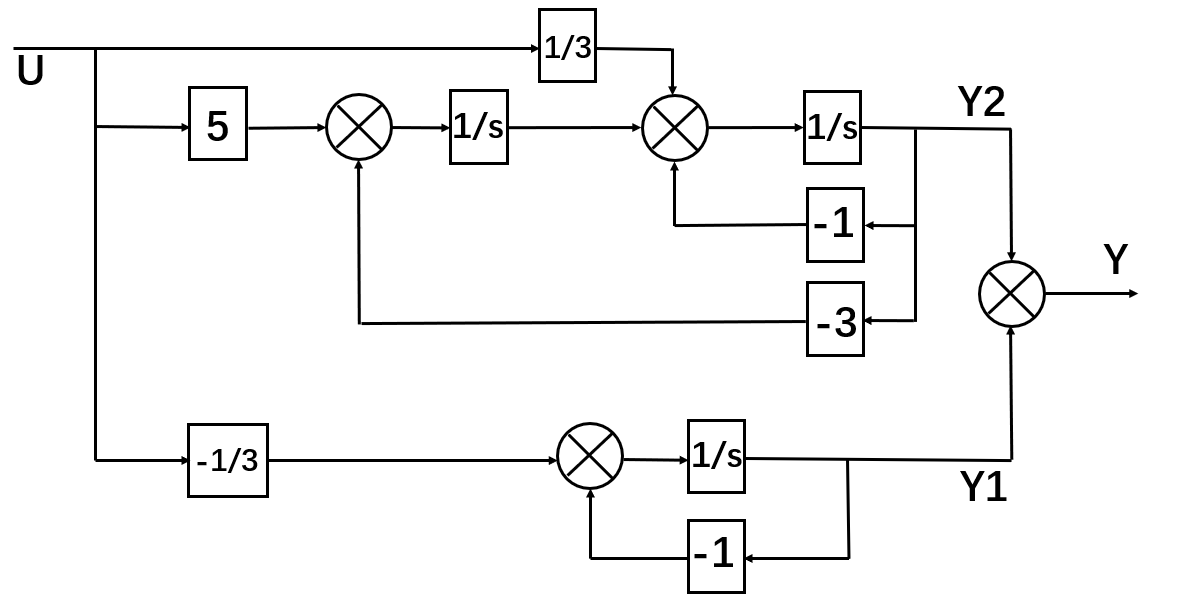
\includegraphics[width=0.7\linewidth]{10}
	\caption{Переход от ПФ к СС}
	\label{fig:10}
\end{figure}
\begin{figure}
	\centering
	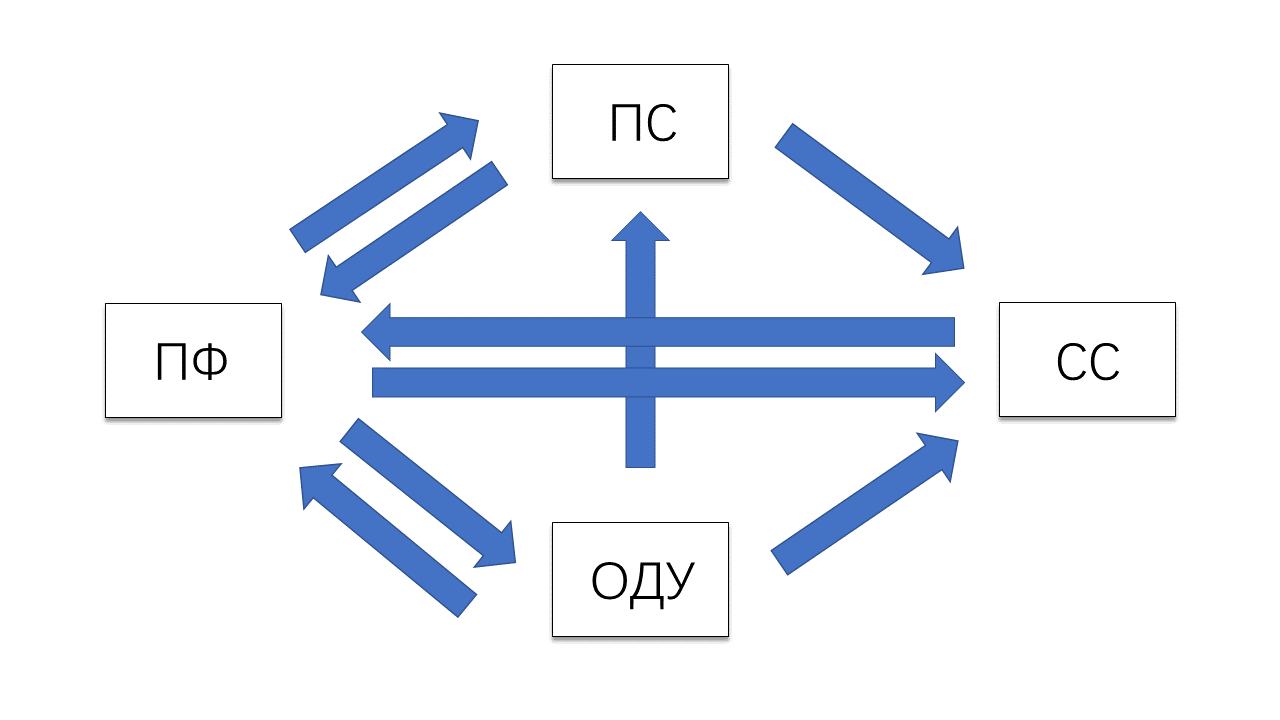
\includegraphics[width=0.7\linewidth]{6}
	\caption{Переходы ЛССНКС}
	\label{fig:6}
\end{figure}
\section{Анализ свойств линейных динамических систем}
\subsection{Статические характерисики}
\begin{equation}
y(t)=y_{\text{п}}(t)+y_{\infty}(t)
\end{equation}
$y_{\text{п}}(t)$ - \emph{переходная режим}, поведение при $t\in[0,T]$.\\
$y_{\infty}(t)$ - \emph{установившийся режим}, поведение при $t\in [T,\infty)$.\\
Статическая характеристика - устанавливает связь между входом и выходом динамической системы а установившемся режиме. 
\subsubsection{Нахождение установившегося режима}
Предположения:\\
1. $x(0)=0$.\\
2. Типовые входные сигналы.
\begin{itemize}
	\item Постоянный сигнал: $u(t)=1$. 
	\item Функция Хевисаида.
	\begin{equation*}
	u(t)=\mathcal{X}(t)=\left\{\begin{array}{cc}
	1,\quad t\ge 0,\\
	0,\quad t<0.
	\end{array}\right.
	\end{equation*}
	\item Полиномиальный сигнал
	\begin{equation*}
	u(t)=u_0+u_1t+\ldots+u_kt^k, \quad k=0,1,2\ldots
	\end{equation*}
	\item Гармонический сигнал
	\begin{equation*}
	u(t)=A\sin\omega t,\quad u(t)=u_0e^{i\omega t}
	\end{equation*}
	\item Дельта-функция
	\begin{equation*}
	u(t)=\delta(t)=\left\{\begin{array}{cc}
	0,\quad t\ne 0,\\
	+\infty,\quad t=0.
	\end{array}\right.\\
	\end{equation*}
	\subitem $\int_{-\infty}^{\infty} \delta(t)dt =1$
	\subitem $\int_{0}^{t}f(\tau)\delta(t-\tau)d\tau=f(t)$
	\subitem пример: при $n\rightarrow\infty$ получим $\delta(t)$.
	\begin{equation*}
	u_n(t)=\left\{\begin{array}{cc}
	n,\quad t\in(0,1/n),\\
	0,\quad t\notin[0,1/n).
	\end{array}\right.\\
	\end{equation*}
\end{itemize}

\textbf{Способ нахождения установившегося режима}
\begin{itemize}
	\item $u(t)\equiv 1,\quad y_{\infty}(t)=\lim_{t\rightarrow\infty}y(t)$.
	\item Вход полиномиального типа $u(t)=u_0+u_1(t)+\ldots+u_lt^l$\\
	\begin{equation*}
	y_{\infty}(t)=\sum_{k=0}^{l+1}c_ku^{(k)},\quad c_k=\frac{1}{k!}\frac{d^kW(s)}{ds^k}\bigg|_{s=0}
	\end{equation*}
	\item Для всех типовых сигналов\\
	Пусть\\
	$D_1 = \sum \{\text{простейшие дроби со знаменателем в } \mathbb{C}_{-}\}$,\\
	$D_2=\sum \{\text{простейшие дроби со знаменателем} \in Im(s)\}$.\\
	Тогда
	\begin{equation}
	Y(s)=W(s)U(s)=D_1+D_2=\{\mathcal{L}^{-1}\}= y_{\text{п}}(t)+y_{\infty}(t)
	\end{equation}
\end{itemize}

\subsection{Динамические характерисики(Временные функции)}
Динамическая характерисика - описывает поведение линейного объекта (системы) в переходном режиме.
\subsubsection{Весовая(импульсная) функция и переходная функция}
\textbf{Весовая (импульсная) функция} $k(t)$- выход системы при нулевых начальных условиях и входном сигнале в виде мгновенного единичного импульса.\\
\textbf{Переходная функция} $h(t)$ - выход системы при нулевых начальных условиях и единичном входном сигнале.\\
\subsubsection{Вычисление динамических характеристик}
\begin{equation}
\begin{aligned}
k(t)&=c\int_{0}^{t}e^{A\tau}\delta(t-\tau)d\tau\cdot b=ce^{At}b\\
h(t)&=x\int_{0}^{t}e^{A(t-\tau)}\mathcal{X}(\tau)d\tau\cdot b=cA^{-1}(e^{At}-I)b
\end{aligned}
\end{equation}
\begin{equation}
\begin{aligned}
\bm{\mathcal{L}\{k(t)\}}&=\bm{W(s),\quad \mathcal{L}\{h(t)\}=W(s)1/s,\quad h'(t)=k(t)}\\
\text{При }Y&=W_1W_2U:\\
k(t)&=\mathcal{L}^{-1}\{W_1W_2\}=(k_1\cdot k_2)(t)\\
h(t)&=\mathcal{L}^{-1}\{(W_1W_2)/s\}=(h_1\cdot h_2)(t)\\
\text{При }Y&=(W_1+W_2)U:\\
k(t)&=\mathcal{L}^{-1}\{W_1+W_2\}=k_1(t)+ k_2(t)\\
h(t)&=\mathcal{L}^{-1}\{(W_1+W_2)/s\}=h_1(t)+h_2(t)\\
\end{aligned}
\end{equation}
\subsection{Частотная характеристика}
Комплекснозначная функция $W(i\omega),\omega\in[0,+\infty)$ называется \emph{частотной характеристикой} системы $Y(s)=W(s)U(s)$.
\begin{equation}
W(i\omega)=\rho(\omega)e^{i\varphi(\omega)}
\end{equation}
$\rho(\omega)$ - \emph{амплитудно-частотная характеристика} (АЧХ).\\
$\varphi(\omega)$ - \emph{фазово-частотная характеристика} (ФЧХ).\\
\subsubsection{Годограф}
Годограф - кривая, описываемая концом вектора $W(i\omega)$ при изменении частоты $\omega$ от $0$ до $\infty$.  
\subsubsection{Вычисление амплитудно-частотной и фазовой характеристик}
Пример
\begin{equation}
\begin{aligned}
W(s)&=\frac{s+1}{(s+2)(s+3)}\\
W(i\omega)&=\frac{i\omega +1}{(i\omega +2)(i\omega +3)}\\
\rho(\omega)&=|W(i\omega)|=\frac{\sqrt{1+\omega^2}}{\sqrt{4+\omega^2}\sqrt{9+\omega^2}}\\
\varphi(\omega)&=\arg W(i\omega)=\arg (i\omega+1)-\arg(i\omega+2)-\arg(i\omega+3)
\end{aligned}
\end{equation}
\subsection{Устойчивость полиномов}
Полином $\alpha(s)=a_0+a_1s+\ldots+a_ns^n$ \textbf{устойчив}, если все его корни лежат строго в левой полуплоскости.\\
\textbf{Необходимое условие устойчивости} Если $\alpha(s)$ устойчив, то все его коэффициенты имеют один и тот же знак.\\
\textbf{Теорема} Для полиномов 1-й и 2-й степени необходимое условие является и достаточным.\\
\textbf{Теорема} Устойчивость $\alpha(s)$ эквивалентна устойчивости полинома $\bar{\alpha}(s)=s^n\alpha\left(\frac{1}{s}\right)=a_0s^n+a_1s^{n-1}+\ldots+a_n(a_i>0)$. Т.е. $\alpha(s)$ устойчив $\Leftrightarrow\bar{\alpha}(s)$ устойчив.
\subsubsection{Критерий Гурвица}
Пусть $a_i>0$. $\alpha(s)$ устойчив $\Leftrightarrow$ главные диагональные миноры матрицы Гурвица $M_n$ положительны.\\
\emph{Матрица Гурвица} строится следующем образом: в каждой строке записываются коэффициенты полинома, начиная c $a_{2n+1}$, в порядке убывания их номеров. Элементы, которые расположены после $a_0$ записываются нулями.
\begin{equation} 
M_n=\left(\begin{array}{ccccccc}
a_1&a_0&0&0&0&\ldots&0\\
a_3&a_2&a_1&a_0&0&\ldots&0\\
a_5&a_4&a_3&a_2&a_1&\ldots&0\\
\ldots&\ldots&\ldots&\ldots&\ldots&\ldots&\ldots\\
a_{2n+1}&a_{2n}&a_{2n-1}&\ldots&\ldots&\ldots&a_n\\
\end{array}\right)
\end{equation}
\subsubsection{Критерий Рауса}
Полином $\alpha(s)$ устойчив $\Leftrightarrow$ 1-й столбец таблицы Рауса содержит только положительные элементы.\\
\emph{Таблица Рауса} составляется следующим образом:
\begin{itemize}
	\item В первой строке записываются коэффициенты уравнения с четными индексами в порядке их возрастания.
	\item Во второй строке - с нечетными.
	\item Остальные элементы таблицы определяется по формуле:
	\begin{equation}
	c_{kl}=c_{k-2,l+1}-r_kc_{k-1,l+1},r_k=\frac{c_{k-2,1}}{c_{k-1,1}},k=3,4,\ldots;l=1,2,\ldots
	\end{equation}
	То есть $r_k$ равно отношению элементов предыдущих двух строк первого столбца. $c_{kl}$ равен разности элементов предыдущих двух строк следующего столбца, притом вычитаемое умножается на $r_k$.
	\item Таблица Рауса содержит $n+1$ строку. Число столбцов убывает при росте номера строки. Элементы, не принадлежащие первому столбцу вычисляются по необходимости.
\end{itemize}
\begin{table}[]
	\label{1}
	\centering
	\begin{tabular}{|c|c|c|c|c|}
		\hline
		No.& 1&2&3&\ldots  \\ \hline
		1 &    $c_{11}=a_0$ & $c_{12}=a_2$ &    $c_{13}=a_4$   &\ldots        \\ \hline
		2 &   $c_{21}=a_1$&  $c_{22}=a_3$   &   $c_{23}=a_5$   &\ldots        \\ \hline
		3 & $c_{31}=c_{12}-r_3c_{22}$& $c_{32}=c_{13}-r_3c_{23}$ &    $c_{33}=c_{14}-r_3c_{24}$   &  \ldots      \\ \hline
		4&        $c_{41}=c_{22}-r_4c_{32}$ & $c_{42}=c_{23}-r_4c_{33}$     &   $c_{43}=c_{24}-r_4c_{34}$       &   \ldots      \\ \hline
		\ldots&        \ldots    &  \ldots    &   \ldots       &  \ldots         \\ \hline
		$n+1$&      $c_{n+1}=c_{n-1,2}-r_{n+1}c_{n2}$  & & &      \\ \hline
	\end{tabular}
\end{table}
\subsubsection{Принцип аргумента}
\textbf{Теорема} $\Delta \arg_{0\le\omega\le\infty}\alpha(i\omega)=\frac{\pi}{2}(n-2l)$, где $l$ - число нулей полинома, лежащих в правой полуплоскости, $n-l$ -  число нулей полинома, лежащих в левой полуплоскости.
\subsubsection{Критерий Михайлова}
$\alpha(s)$ устойчив $\Leftrightarrow\Delta\arg_{0\le\omega\infty}\alpha(i\omega)=\frac{\pi}{2}n,\quad n=\deg\alpha(s)$.\\
Следствие. Если $\alpha(s)$ устойчивый, то $\varphi(\omega)=\arg\alpha(i\omega)$ - строго монотонная функция
\subsection{Устойчивость линейных динамических объектов}
\begin{equation}
\left\{\begin{array}{cc}
\dot{x}=Ax+bu\\
y=cx
\end{array}\right.\\
\end{equation}
Объект \emph{устойчив} (по состоянию), если при $u\equiv0,\forall x(0)\Rightarrow\|x(t)\|\rightarrow0$ при $t\rightarrow\infty$.
\subsubsection{Критерий устойчивости в ПС}
Объект устойчив $\Leftrightarrow \sigma(A)\subset \mathbb{C}_{-}$
\subsubsection{Критерий устойчивости по ПФ}
$W(s)=\frac{\beta(s)}{\alpha(s)}$ устойчив $\Leftrightarrow$ $\alpha(s)$ устойчив.
\subsubsection{Критерий устойчивости по весовой функции}
$y(t)=\int_{0}^{\tau}k(t-\tau)u(\tau)d\tau$ устойчив $\Leftrightarrow$ весовая функция объекта абсолютно интегрируема по оси $(0,+\infty)$, т.е. $\int_{0}^{\infty}|k(\tau)|d\tau<const$.
\subsection{Управляемость линейных динамических объектов} 
\begin{equation}
\left\{\begin{array}{cc}
\dot{x}=Ax+bu\\
y=cx
\end{array}\right.
\end{equation}
Объект \emph{управляем} по состоянию, если: \\для $\forall x_0,x_1\in\mathbb{R}^n,\forall T_0>0,\exists u_{[0,T_0]}:
\left\{\begin{array}{cc}
	x(0)=x_0\\
	x(T_0)=x_1
\end{array}\right.$
\subsubsection{Критерий управляемости}
$K_{A,b}=[b\,Ab\,A^2b\,\ldots\,A^{n-1}b]\in\mathbb{R}^n$ - \emph{Матрица управляемости}.\\
\textbf{Критерий управляемости} Объект управляемый $\Leftrightarrow\,\operatorname{rank}K_{A,b}=n$.
\subsubsection{Каноническая форма управляемости}
Эта форма удобна для построения модального управления.
\begin{equation}
\left\{\begin{array}{cc}
\dot{z}=\bar{A}x+\bar{b}u,\\
y=\bar{c}x.\\
\end{array}\right.
\end{equation}
где $\bar{A}=MAM^{-1},\bar{b}=Mb=(0,\ldots,1)^T,\bar{c}=cM^{-1},|M|\ne0$.
\begin{equation} 
\bar{A}=\left(\begin{array}{ccccc}
0&1&0&\ldots&0\\
0&0&1&\ldots&0\\
\ldots&\ldots&\ldots&\ldots&\ldots\\
0&0&0&\ldots&1\\
-a_0&-a_1&-a_2&\ldots&-a_{n-1}\\
\end{array}\right)
\end{equation}
В этом случае справедливо $K_{\bar{A},\bar{b}}=MK_{A,b}$.\\
\textbf{Критерий управляемости} \\Объект управляемый $\Leftrightarrow\,\operatorname{rank}K_{A,b}=n\Leftrightarrow\operatorname{rank}K_{\bar{A},\bar{b}}=n$.
\subsubsection{Модальное управление. Стаблизация по состоянию линейного объекта} 
\textbf{Задача стаблизации} Для объекта построить обратную связь.\\
$u=u(x):x=Ax+bu(x)$.\\
\textbf{Модальное управление по состоянию} линейного динамического объекта\\
Выбор обратной связи по состоянию следующим типом:\\
$u=-kx:\dot{x}=(A-bk)x.\quad \sigma(A-bk)$ - заданный спектр.\\
\textbf{Задача стаблизации объекта методами модальной стаблизации}\\
Выбор линейной обратной связи вида $-kx$, обеспечивающей заданной системе заданный спектр, лежащий в левой полуплоскости.\\
\textbf{Алгоритм стаблизации модальным управлением}
\begin{enumerate}
	\item построить $K_{A,b}$ и проверить $\operatorname{rank}K_{A,b}=n$
	\item построить $x_{A}(s)=s^n+a_{n-1}s^{n-1}+\ldots+a_0$
	\item построить $K_{\bar{A},\bar{b}}$
	\item $M=K_{\bar{A},\bar{b}}\cdot K_{A,b}^{-1}$
	\item построить полином с заданным спектром: $\gamma(s)=(s-s_1)\ldots(s-s_n)=s^n+\gamma_{n-1}s^{n-1}+\ldots+\gamma_0$
	\item вычислять $\bar{k}_i=\gamma_{i-1}-a_{i-1},\quad i=1,\ldots,n$
	\item получим $k=\bar{k}M$ 
\end{enumerate}
\subsection{Наблюдаемость линейных динамических объектов} 
\begin{equation}
\left\{\begin{array}{cc}
\dot{x}=Ax+bu\\
y=cx
\end{array}\right.
\end{equation}
Объект \emph{наблюдаем}, если при $u\equiv0,\,\forall x_1(0)\ne x_2(0)\Rightarrow y(t,x_1(0))\not\equiv y(t,x_2(0))$. То есть между входом и выходом можно восстановить однозначное соответствие, через которое по выходу $y(t)$ можно наблюдать начальное состояние системы $x(0)$.
\subsubsection{Критерий наблюдаемости}
$N_{c,A}=\left(\begin{array}{c}
c\\cA\\\ldots\\cA^{n-1}
\end{array}\right)$ -\emph{Матрица наблюдаемости}.\\
\textbf{Критерий наблюдаемости} Объект наблюдаем $\Leftrightarrow\,\operatorname{rank}N_{c,A}=n$.\\
\textbf{Оценка вектора состояний }(Как выразить $x(t)$ через $y(t),\ldots,y^{(n-1)}(t)$)\\
\begin{equation}
\begin{aligned}
y&=cx\\
\dot{y}&=c\dot{x}=cAx+cbu\\
\ddot{y}&=cA\dot{x}+cb\dot{u}=cA^2x+cAbu+cb\dot{u}\\
&\ldots\quad\ldots\quad\ldots\\
\Rightarrow\left(\begin{array}{c}
y(t)\\\ldots\\y^{(n-1)}(t)
\end{array}\right)&=N_{c,A}\left(\begin{array}{c}
x_1(t)\\\ldots\\x_n(t)
\end{array}\right)+\left(\begin{array}{c}
cbu\\cAbu+cb\dot{u}\\\ldots\\cA^{n-2}bu+\ldots+cbu^{(n-2)}
\end{array}\right)
\end{aligned}
\end{equation}
Пусть второе слагаемое обозначается как $\psi(t)$, тогда
\begin{equation}
\left(\begin{array}{c}
x_1(t)\\\ldots\\x_n(t)
\end{array}\right)=N_{c,A}^{-1}\left(
\left(\begin{array}{c}
y(t)\\\ldots\\y^{(n-1)}(t)
\end{array}\right)
+\psi(t)\right)
\end{equation}
\subsubsection{Каноническая форма наблюдаемости}
Эта форма удобна для построения наблюдателя Люенбергера.
\textbf{Теорема} Пусть линейный объект вполне наблюдаемый. Тогда существует такое невырожденное линейное преобразование а пространстве состояний $z=Tx,T\in\mathbb{R}^{n\times n}$, что система в переменных $z$ имеет вид 
\begin{equation}
\left\{\begin{array}{cc}
\dot{z}=\bar{A}z+\bar{b}u\\
y=\bar{c}z
\end{array}\right.\\
\end{equation}
где
\begin{equation} 
\bar{A}=\left(\begin{array}{ccccc}
0&0&\ldots&0&-a_0\\
1&0&\ldots&0&-a_1\\
0&1&\ldots&0&-a_2\\
\ldots&\ldots&\ldots&\ldots&\ldots\\
0&0&\ldots&1&-a_{n-1}\\
\end{array}\right)
\end{equation}
\begin{equation*}
c=(0,\ldots,1)
\end{equation*}
В этом случае справедливо $N_{\bar{c},\bar{A}}=T^{-1}N_{c,A}$
\subsubsection{Наблюдатель, наблюдатель Люенбергера}
\emph{Наблюдателем} для системы будем называть любое преобразование $\bar{x}=N(u,y)$, для которого выходная переменная $\bar{x}$ удовлетворяет одному из двух условий.
\begin{enumerate}
	\item $|x-\bar{x}|<\varepsilon$ для некоторого $\varepsilon>0$ при всех $t\ge t_0\ge 0$.
	\item $|x-\bar{x}|\rightarrow 0$ при $t\rightarrow\infty$. В этом случае наблюдатель называется \emph{асимптотическим}.
\end{enumerate}
\emph{Асимптотический наблюдатель Люенбергера} - система дифференциальных уравнений вида
\begin{equation*}
\dot{\bar{x}}=A\bar{x}+l(y-c\bar{x})+bu,\quad l\in\mathbb{R}^{n\times 1}
\end{equation*}
Тогда пусть $e_x(t)=x(t)-\bar{x}(t)$ - ошибка наблюдения, имеем
\begin{equation*}
\dot{e_x}=(A-lc)e_x
\end{equation*}
При устойчивой системе про $e_x$ имеем стремление к нулю ошибки, то есть $\sigma(A-lc)\in\mathbb{C}_{-}$. Теорема о назначении спектра наблюдателя Люенбергера говорит нам о том, что всегда найдется вектор $l$ такой, что $\sigma(A-lc)=\Lambda$, где $\Lambda$ - заданный спектр.\\
\textbf{Алгоритм построения наблюдателя Люенбергера}
\begin{enumerate}
	\item построить $N_{c,A}$ и проверить $\operatorname{rank}N_{c,A}=n$
	\item построить $x_{A}(s)=s^n+a_{n-1}s^{n-1}+\ldots+a_0$
	\item построить полином с заданным спектром: $\gamma(s)=(s-s_1)\ldots(s-s_n)=s^n+\gamma_{n-1}s^{n-1}+\ldots+\gamma_0$
	\item построить $N_{\bar{c},\bar{A}}$
	\item построить $T=N_{\bar{c},\bar{A}}^{-1}\cdot N_{cA}$
	\item вычислять $\bar{l}_i=\gamma_{i-1}-a_{i-1},\quad i=1,\ldots,n$
	\item получим $l=T^{-1}\bar{l}$ 
\end{enumerate}
\subsection{Полиномиальная стаблизация}
Пусть имеем систему с передаточной функцей 
\begin{equation*}
W(s)=\frac{\beta(s)}{\alpha(s)}
\end{equation*}
Требуется построить регулятор с передаточной функцией $R(s)=\frac{p(s)}{q(s)}$, при замыкании которым систему получить желаемый устойчивый спектр матрицы, то есть
\begin{equation*}
W_c(s)=\frac{W(s)}{1+W(s)R(s)}=\frac{\beta(s)q(s)}{\alpha(s)q(s)+\beta(s)p(s)}
\end{equation*}
Нужно выбрать полиномы $p(s),q(s)$ так, чтобы $\alpha(s)q(s)+\beta(s)p(s)$ устойчива. Обычно положим $\deg q(s)=n-1,\deg p(s)\leqslant n-1,\quad n$ - степень полинома $\alpha(s)$.\\
\end{document}

